\documentclass{article}
\usepackage[utf8]{inputenc}
\usepackage{amsmath,amsfonts,amssymb}
\usepackage[margin=1in]{geometry}
\usepackage[parfill]{parskip}
\usepackage{authblk} % Better formatting of affiliations.
\usepackage{graphicx} % Allow graphics
\usepackage{xcolor} % Allow colored text.

% for nice url formatting, including auto linebreaks
\usepackage{xurl}

% makes nice looking tables
\usepackage{tabularx}

% get periods in figure captions instead of colons
\usepackage[labelsep=period]{caption}

% indicate FIXMEs with red text
\newcommand{\fixme}[1]{{\color{red}{#1}}}

\title{
  \textbf{Supporting Information} \bigskip \bigskip \bigskip \bigskip \\
  Evaluating proteomics imputation methods with improved criteria}

\author[1]{Lincoln Harris}
\author[2]{William E.\ Fondrie}
\author[3]{Sewoong Oh}
\author[1,3,*]{William S.\ Noble}

\affil[1]{Department of Genome Sciences, University of Washington,  Seattle, Washington, 98195, United States}
\affil[2]{Talus Biosciences, Seattle, Washington, 98112, United States}
\affil[3]{Paul G.\ Allen School of Computer Science and Engineering,
  University of Washington, Seattle, Washington, 98195, United States}
\affil[*]{Corresponding author. Email: william-noble@uw.edu}

\date{}

\begin{document}

% Label the following figures as supplementary
\appendix
\renewcommand{\figurename}{Supplementary Figure}
\renewcommand{\tablename}{Supplementary Table}
\renewcommand{\thepage}{S-\arabic{page}}
\setcounter{table}{0}
\setcounter{figure}{0}
\setcounter{page}{1}

\maketitle

\clearpage

\clearpage
\section*{Table of Contents}
\textbf{Supplementary Table 1.} Normalization methods applied to the data sets included in this study. \\
\\
\textbf{Supplementary Figure 1.} Distributions of train and test sets following MCAR and MNAR partitioning procedures. \\
\\
\textbf{Supplementary Figure 2.} Comparing the abilities of imputation methods to identify differentially expressed peptides, as a function of missingness fraction. \\
\\
\textbf{Supplementary Figure 3.} Comparing the abilities of imputation methods to identify differentially expressed peptides for a TMT data set. \\
\\
\textbf{Supplementary Figure 4.} Comparing the abilities of imputation methods to identify differentially expressed peptides for a label-free DDA data set. \\
\\
\textbf{Supplementary Figure 5.} Variance of peptide quantifications is greater than expected following imputation. \\
\\
\textbf{Supplementary Figure 6.} Variance of protein quantifications is greater than expected. \\

\clearpage

\begin{table}
  \centering
  \begin{tabular}{llr}
    \hline
    Identifier & Normalization Method & Citation \\
    \hline
    PXD016079 & Subtraction of means & [31] \\
    PXD006109 & MaxLFQ delayed normalization & [32] \\
    PXD014525 & MaxLFQ delayed normalization & [33] \\
    PXD034525 & Median deviation & [34] \\
    PXD014815 & Total ion current & [35] \\
    PXD013792 & Z-score & [36] \\
    PXD014156 & MaxLFQ delayed normalization & [37] \\
    PXD006348 & Z-score & [38] \\
    PXD011961 & Z-score & [39] \\
    CPTAC-S047 & Median shifting of samples followed by median absolute deviation scaling & [40] \\
    CPTAC-S051 & Median shifting of samples followed by median absolute deviation scaling & [41] \\
    PXD007683 & Normalization to the sum of total signal, for each channel & [42] \\
    \hline
  \end{tabular}
  \caption{{\bf Normalization methods applied to the data sets included in this study.} ProteomeXchange (PXD) and CPTAC reference IDs are provided. Spectral processing and normalization were performed by the original authors of each study.}
    \label{tab:normalization-methods}
\end{table}

\begin{figure}
  \centering
  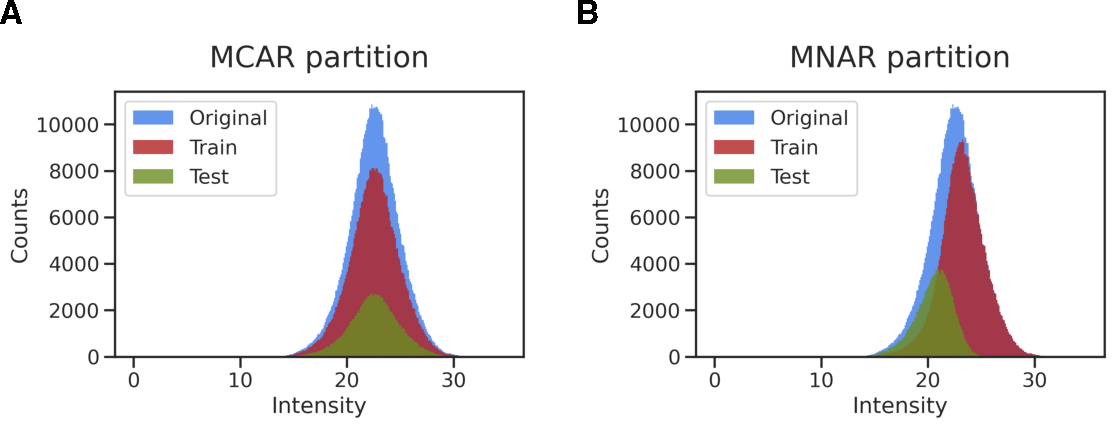
\includegraphics[width=1.0\textwidth]{figures/partition-distributions-figure.pdf}
  \caption{{\bf Distributions of train and test sets following MCAR and MNAR partitioning procedures.} Data were obtained from PXD03452. Log-transformed peptide-level quantifications are shown. 25\% of present matrix entries were selected for the test set.}
  \label{fig:partitions}
\end{figure} 

\begin{figure}
  \centering
  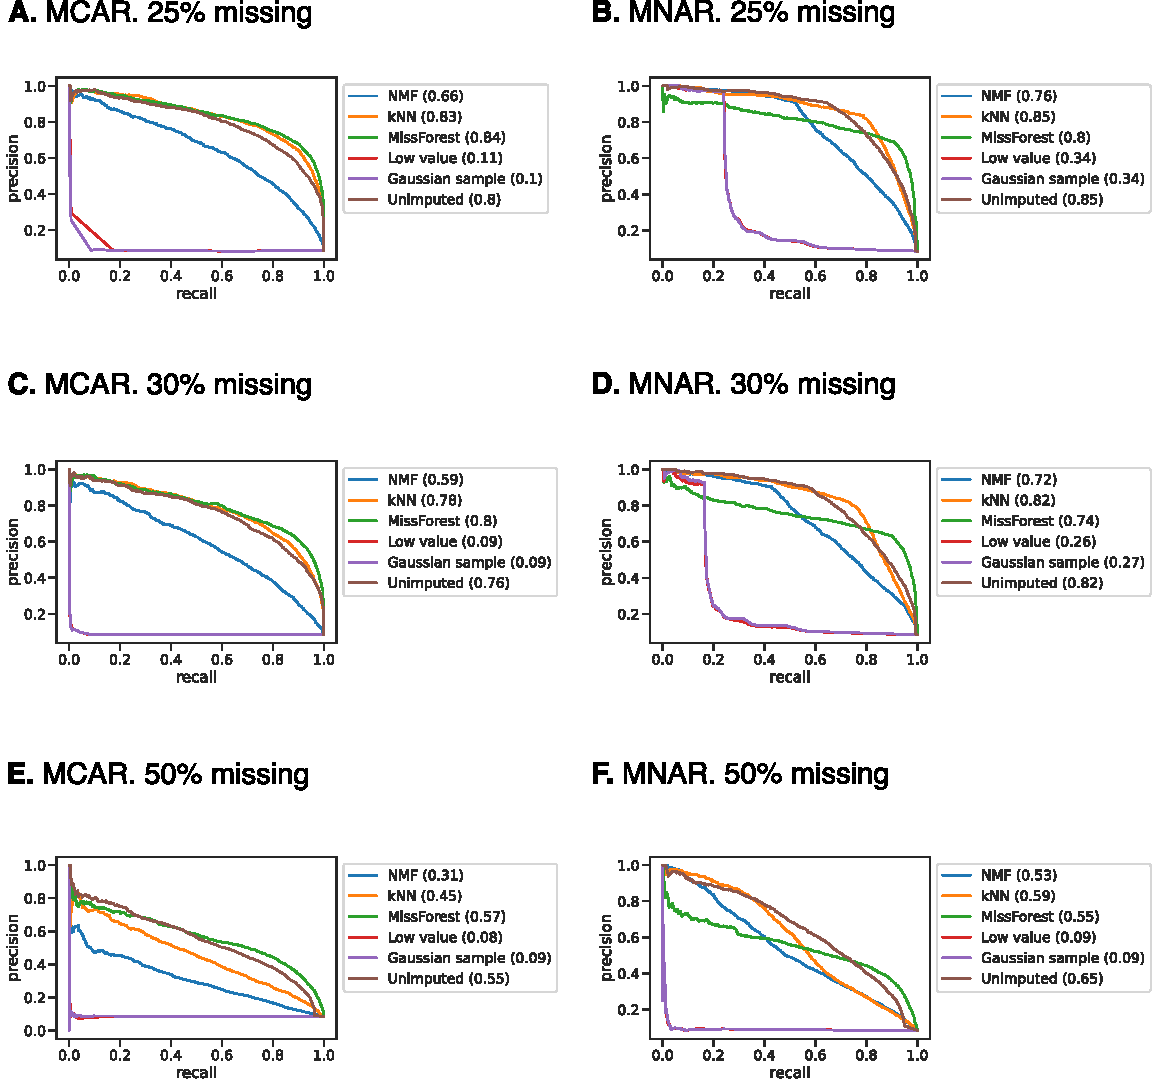
\includegraphics[width=1.0\textwidth]{figures/differential-expression-DIA-extended-figure.pdf}
  \caption{{\bf Comparing the abilities of imputation methods to identify differentially expressed peptides, as a function of missingness fraction.} MCAR and MNAR procedures were used to simulate 25\%, 30\% and 50\% missingness fractions. DIA data were obtained from PXD03452. As described in Figure 3, differentially expressed peptides were identified between two clinically annotated Alzheimer's disease groups. AUC values are shown in parentheses.}
  \label{fig:DE-extended}
\end{figure}

\begin{figure}
  \centering
  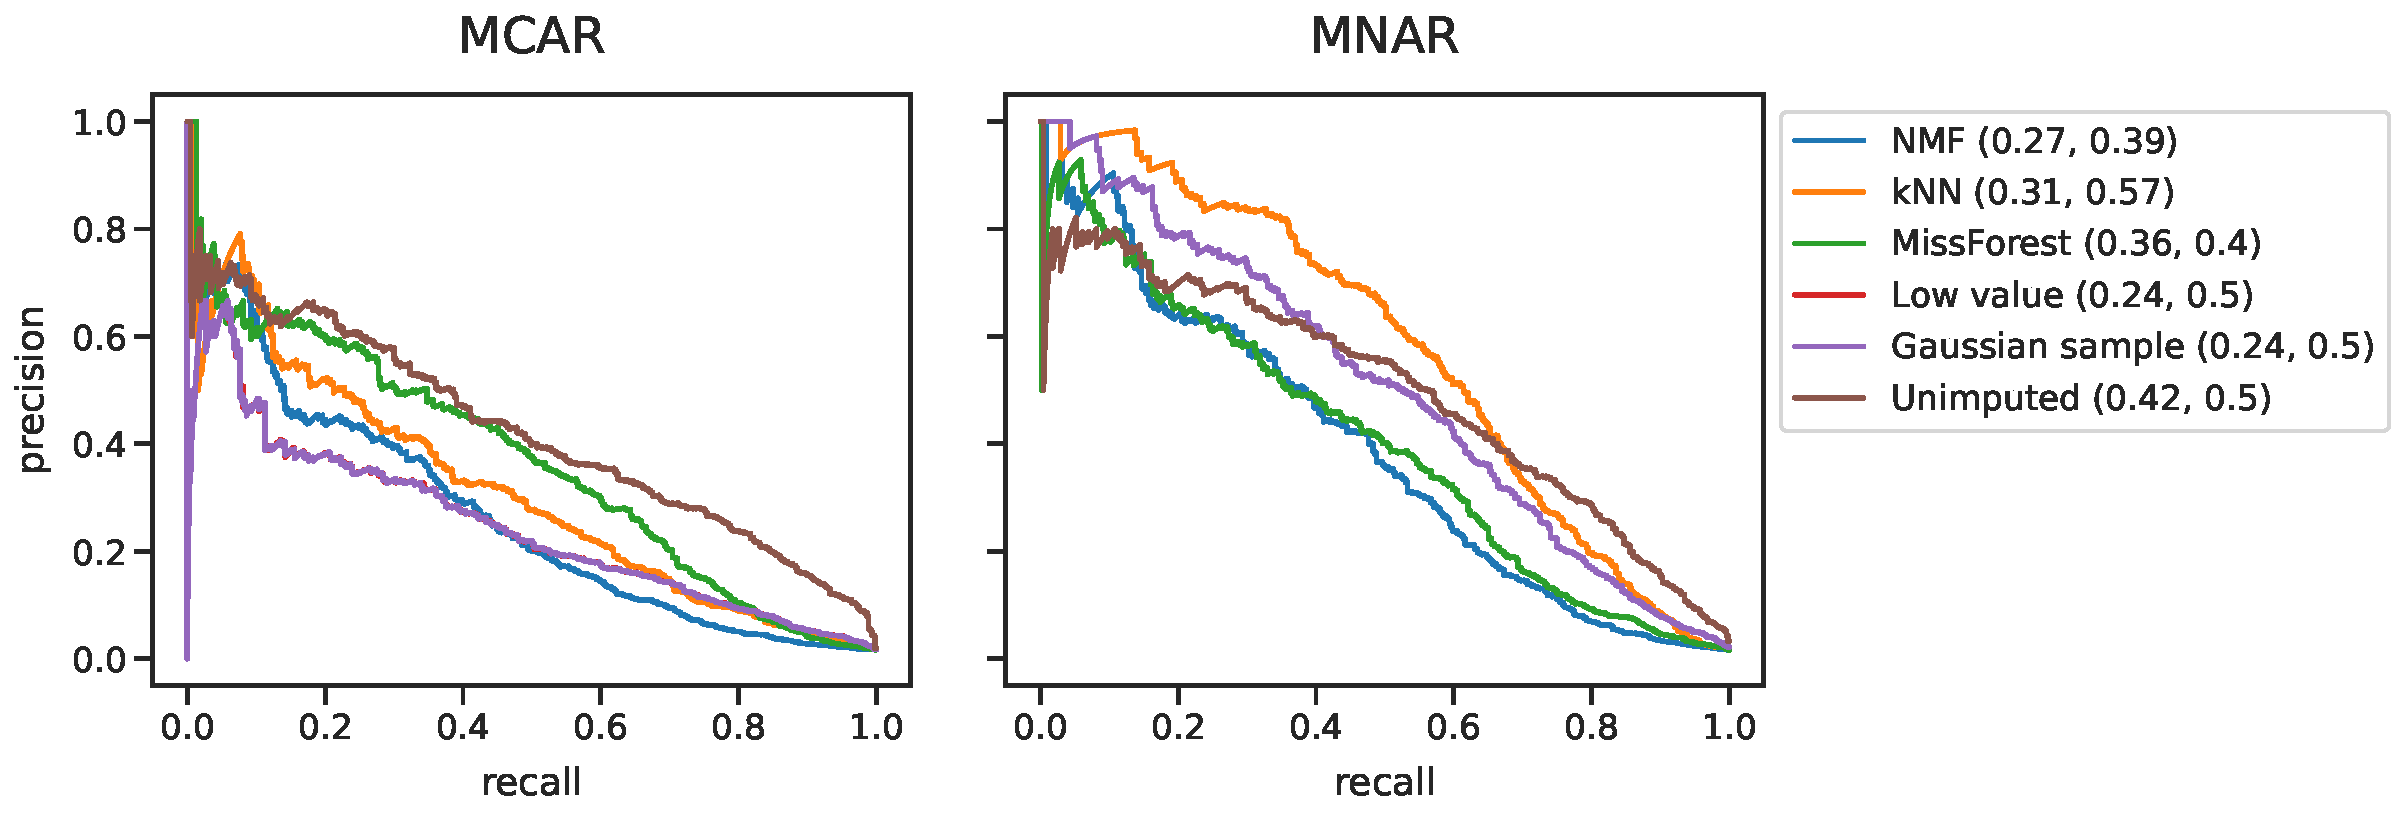
\includegraphics[width=1.0\textwidth]{figures/differential-expression-TMT-figure.pdf}
  \caption{{\bf Comparing the abilities of imputation methods to identify differentially expressed peptides for a TMT data set.} Precision-recall curves are shown for both MCAR and MNAR simulated missingness. Data were obtained from CPTAC-S047; the following clinically annotated groups were compared: ``Low-grade glioma/astrocytoma'' and ``Ependymoma''. AUC values for MCAR and MNAR experiments are given in parentheses.}
  \label{fig:PR-curves-DDA}
\end{figure}

\begin{figure}
  \centering
  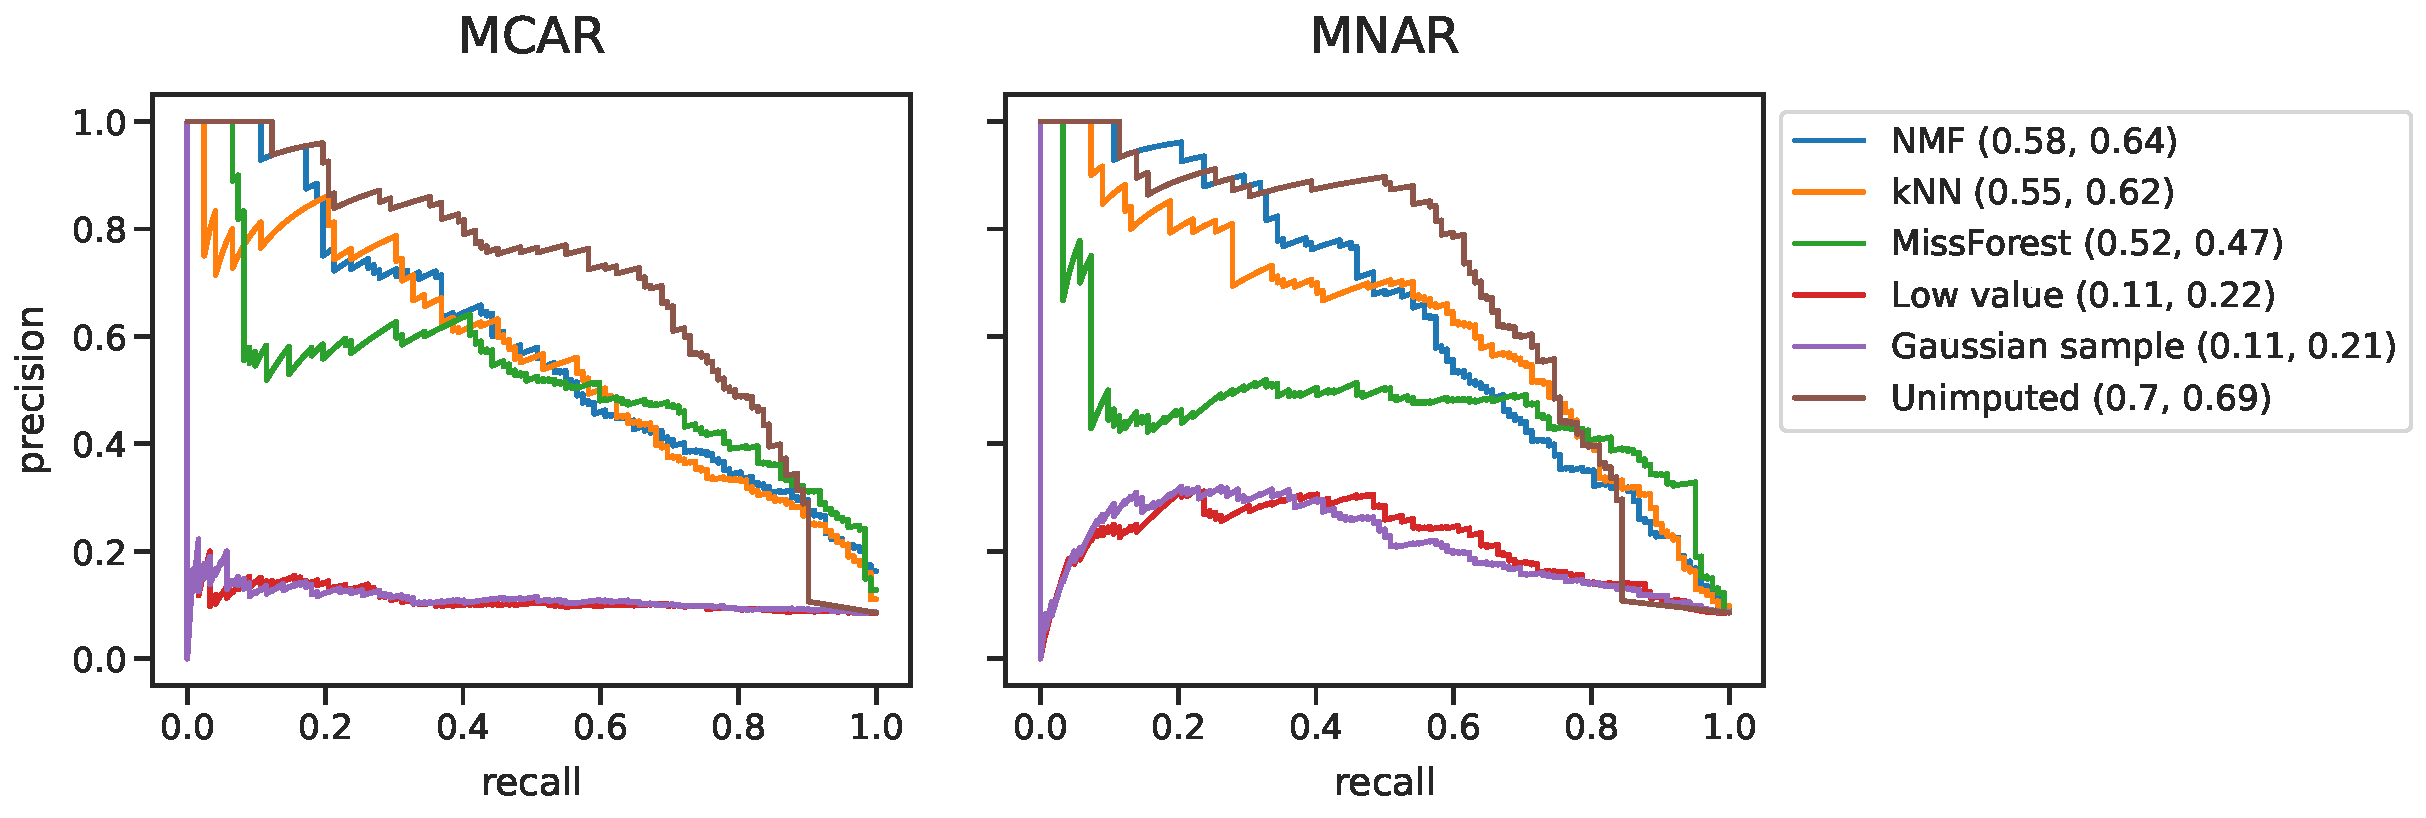
\includegraphics[width=1.0\textwidth]{figures/differential-expression-label-free-DDA-figure.pdf}
  \caption{{\bf Comparing the abilities of imputation methods to identify differentially expressed peptides for a label-free DDA data set.} Precision-recall curves are shown for both MCAR and MNAR simulated missingness. Data were obtained from PXD006348; \textit{Brucella abortus} samples were compared to \textit{Brucella melitensis}. AUC values for MCAR and MNAR experiments are given in parentheses.}
  \label{fig:PR-curves-DDA}
\end{figure}

\begin{figure}
  \centering
  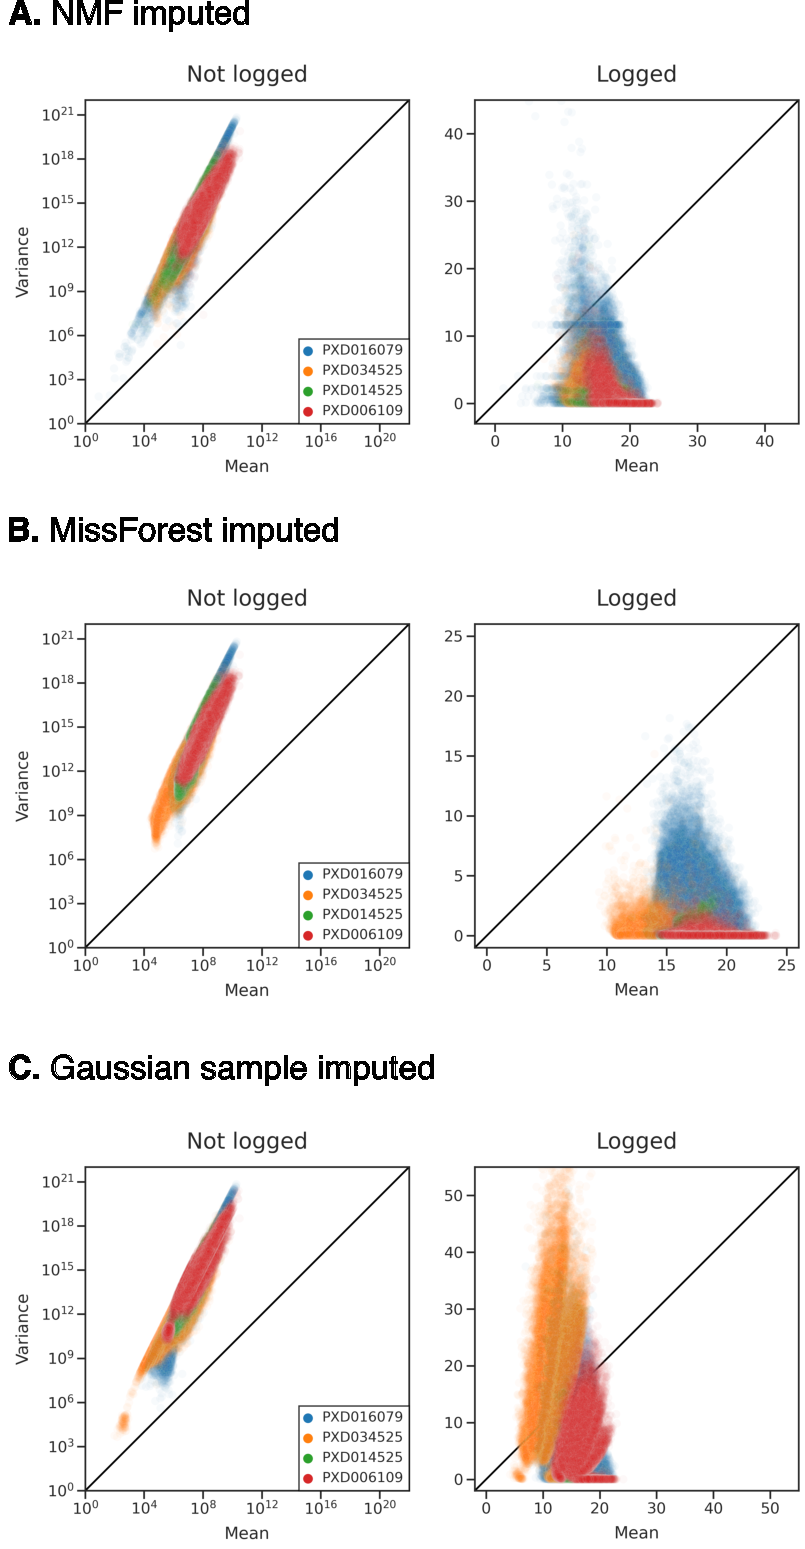
\includegraphics[width=0.6\textwidth]{figures/imputed-distributions.pdf}
  \caption{{\bf Variance of peptide quantifications is greater than expected following imputation.} Four proteomics data sets were imputed with NMF, MissForest and Gaussian sampling. Means and variances were calculated across technical replicates for each imputed peptide, for each data set. In the righthand panels, imputed quantifications have been log-transformed.}
  \label{fig:distributions-post-impute}
\end{figure} 

\begin{figure}
  \centering
  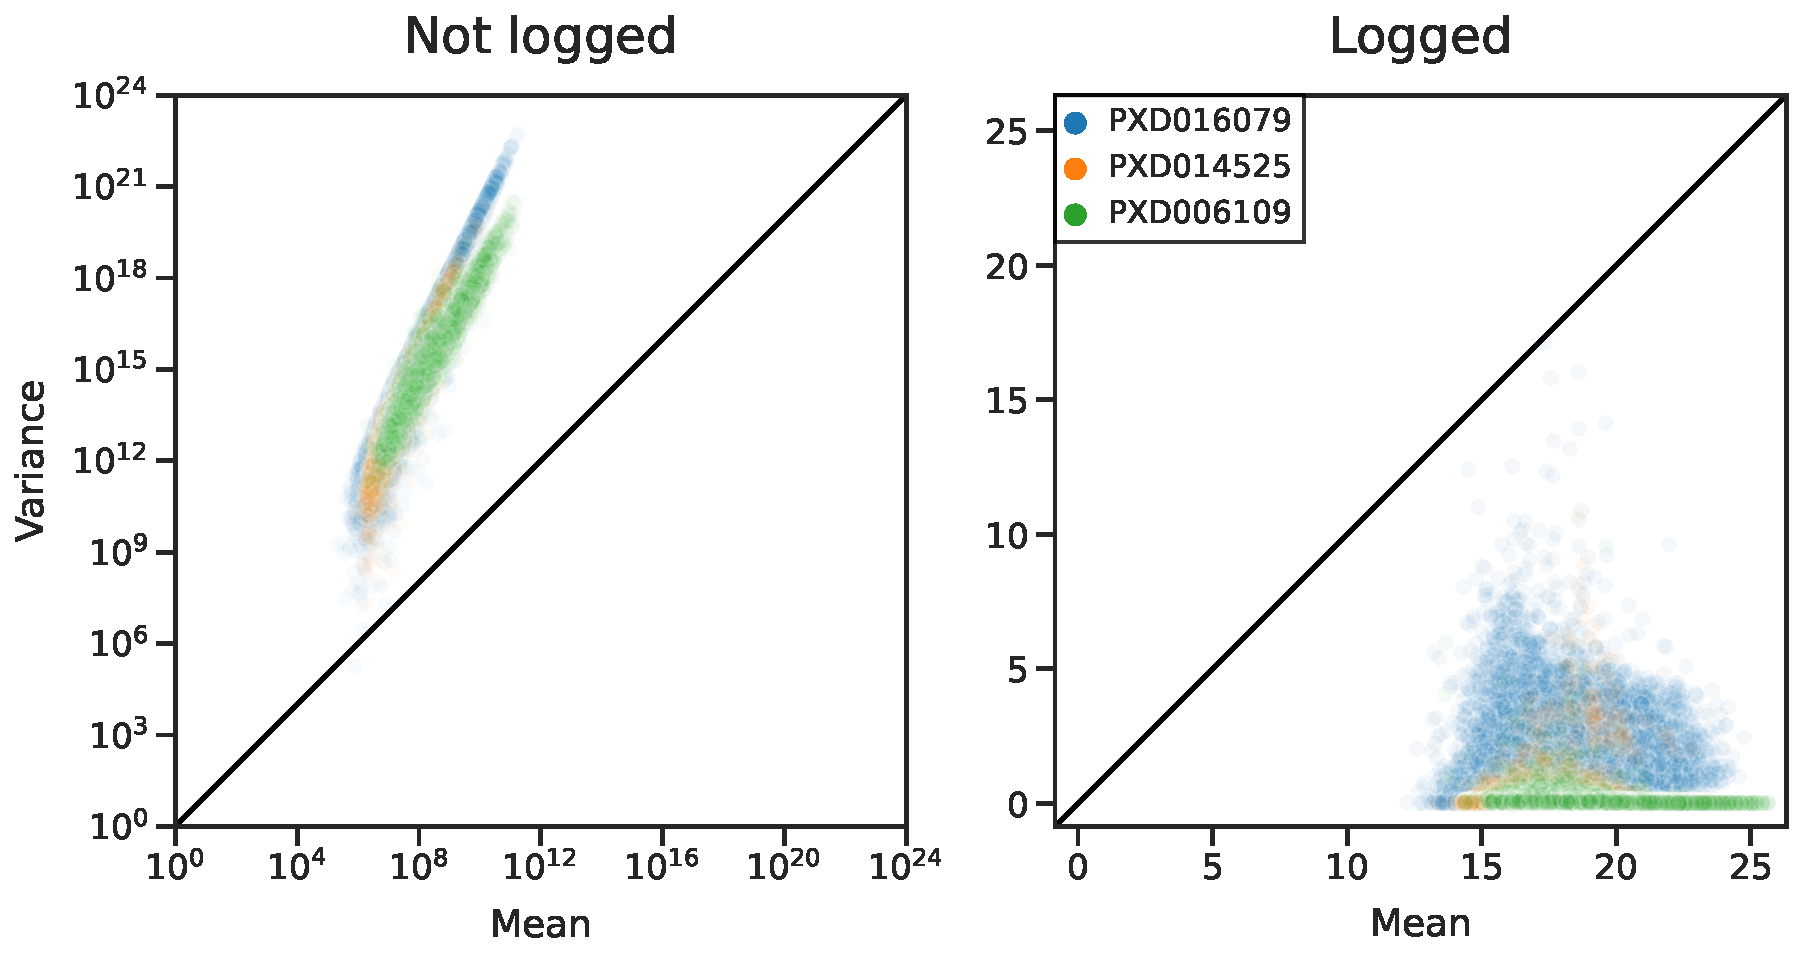
\includegraphics[width=0.7\textwidth]{figures/mean-variance-protein-figure.pdf}
  \caption{{\bf Variance of \textit{protein} quantifications is greater than expected.} Means and variances were calculated across technical replicates for each protein, for three protein-level quantification data sets. In the righthand panel, protein quantifications have been log-transformed.}
  \label{fig:protein-mean-x-var}
\end{figure} 

\end{document}
